\documentclass[13pt, a4paper]{scrartcl}

\usepackage{vorschule}
\usepackage[
    typ=ab,
    fach=Mathematik,
    lerngruppe={Jg.6},
    nummer=3,
    module={Symbole,Lizenzen,Papiertypen},
    seitenzahlen=keine,
    farbig,
    lizenz=cc-by-nc-sa-4,
]{schule}

\usepackage[
	kuerzel=Ngb,
	reihe={Bruchrechnung},
	version={2019-09-8},
]{ngbschule}

\author{J. Neugebauer}
\title{Brüche vergleichen}
\date{\Heute}

\setzeAufgabentemplate{ngbnormal}

\begin{document}

\ReiheTitel

\bigskip
\begin{minipage}{0.79\textwidth}
	Im Moment gibt es in den Ü-Eiern neue Figuren von den \emph{Minions}.
	
	\medskip
	\person{Simon} hat im Schnellkauf \emph{acht Ü-Eier} gekauft. Nachdem er alle geöffnet hat hat er \emph{drei Figuren} gefunden.
	
	\medskip
	\person{Aylin} war im SuperStore und hat dort \emph{12 Eier} im Angebot bekommen. Nach dem Öffnen hat sie \emph{fünf Minion-Figuren}.
\end{minipage} \hfill
\begin{minipage}{0.2\textwidth}
	\begin{center}
		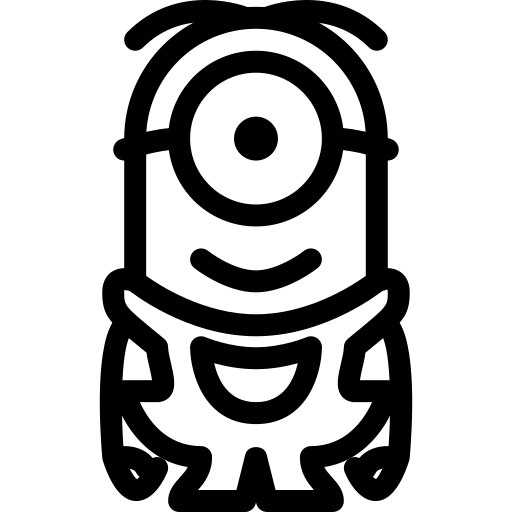
\includegraphics[width=3cm]{6.3-Minion}
	\end{center}
\end{minipage}

\bigskip
\textbf{Wo lohnt es sich nach diesem Test mehr Ü-Eier zu kaufen? Im Schnellkauf oder im SuperStore?}

\begin{teilaufgaben}
	\item Ermittelt für Simon und Aylin aus dem Text den Anteil an Ü-Eiern, die eine Minion-Figur enthielten.
	\item Stellt die Anteile der beiden in den Rechtecken unten grafisch dar. Schätzt, welcher Anteil größer ist.
	
	\begin{center}
		\begin{tikzpicture}
			\geoPolygonzug{(0,0) |- (3,2) |- (0,0)}
			\foreach \i in {1,...,5}{
				\geoPolygonzug[draw=black!25]{(.5*\i,0) -- (.5*\i,2)}
			}
			\foreach \i in {1,...,3}{
				\geoPolygonzug[draw=black!25]{(0,.5*\i) -- (3,.5*\i)}
			}
			\geoPolygonzug{(4,0) |- (7,2) |- (4,0)}
			\foreach \i in {1,...,5}{
				\geoPolygonzug[draw=black!25]{(4+.5*\i,0) -- (4+.5*\i,2)}
			}
			\foreach \i in {1,...,3}{
				\geoPolygonzug[draw=black!25]{(4,.5*\i) -- (7,.5*\i)}
			}
		\end{tikzpicture}
	\end{center}
	\item Verfeinert die Einteilung der Rechtecke aus b) so, dass beide in gleich viele Teile aufgeteilt sind. Zeichnet die neuen Anteile in die Rechtecke unten. Notiert sie daneben auch als Bruch.
	
	\begin{center}
		\begin{tikzpicture}
		\geoPolygonzug{(0,0) |- (3,2) |- (0,0)}
		\foreach \i in {1,...,5}{
			\geoPolygonzug[draw=black!25]{(.5*\i,0) -- (.5*\i,2)}
		}
		\foreach \i in {1,...,3}{
			\geoPolygonzug[draw=black!25]{(0,.5*\i) -- (3,.5*\i)}
		}
		\geoPolygonzug{(4,0) |- (7,2) |- (4,0)}
		\foreach \i in {1,...,5}{
			\geoPolygonzug[draw=black!25]{(4+.5*\i,0) -- (4+.5*\i,2)}
		}
		\foreach \i in {1,...,3}{
			\geoPolygonzug[draw=black!25]{(4,.5*\i) -- (7,.5*\i)}
		}
		\end{tikzpicture}
	\end{center}
	\item Welcher Supermarkt lohnt sich eurer Meinung nach mehr?
	
	\begin{center}
		\linie
	\end{center}
	\item Erklärt: Welche Brüche lassen sich besonders leicht vergleichen?
	\item[\symStern] Erklärt: Wie kann man Brüche im Allgemeinen vergleichen?
	\item[\symStern] Wie haben sich die Brüche von Teil b) zu c) verändert?
\end{teilaufgaben}

\end{document}
